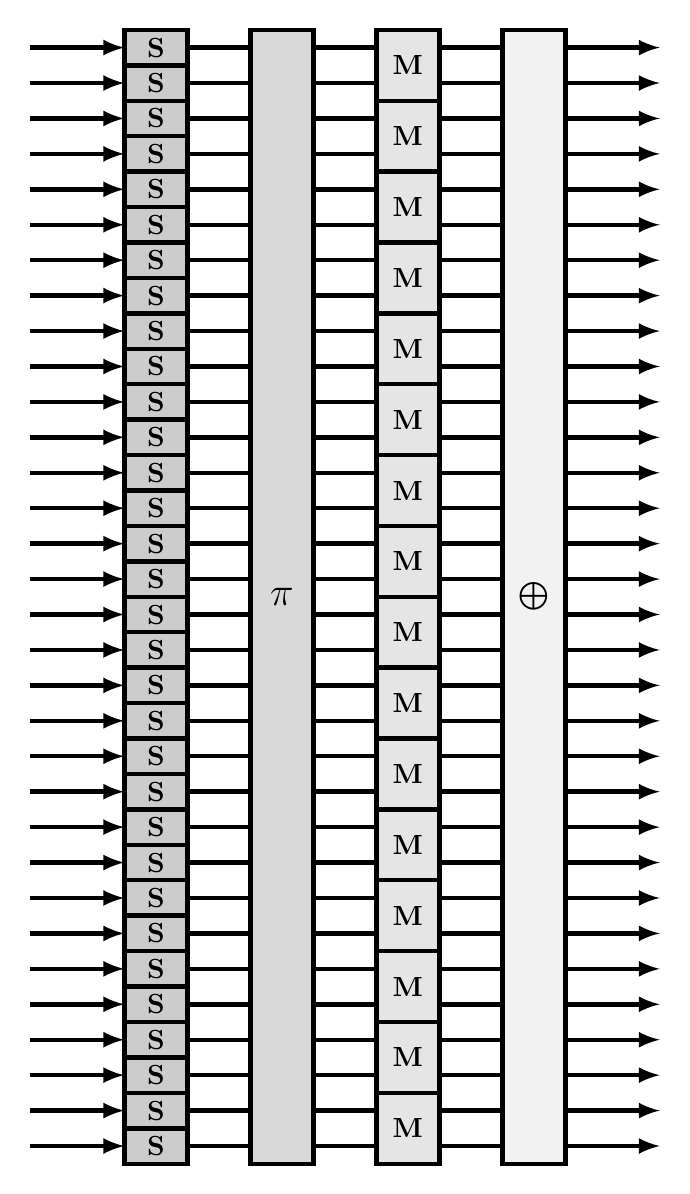
\begin{tikzpicture}[xscale=.8,yscale=0.45,>=latex,ultra thick]
% Reference grid (temporary)
%\draw[help lines] (0,0) grid (16,32);

% TODO label bits / words

% Entry arrows
\foreach \i in {32,...,1} {
  \draw[->] (-1.5,\i-0.5) -- (0,\i-0.5);
}

% Wires
\foreach \j in {1,3,5} {
  \foreach \i in {32,...,1} {
    \draw (\j,\i-0.5) -- (\j+1,\i-0.5);
  }
}

% S-boxes
\foreach \i in {32,...,1} {
  \draw[fill=gray!40] (0,\i) rectangle (1,\i-1) node[midway] {$\mathbf{S}$} ;
}

% P-boxes
\draw[fill=gray!30] (2,0) rectangle (3,32) node[midway] {\Large$\mathbf{\pi}$};

% Mixers
\foreach \i in {32,30,...,2} {
  \draw[fill=gray!20] (4,\i) rectangle (5,\i-2) node[midway] {$\mathbf{M}$};
}

% Round key box
\draw[fill=gray!10] (6,0) rectangle (7,32) node[midway] {$\bigoplus$};

% Exit arrows
\foreach \i in {32,...,1} {
  \draw[->] (7,\i-0.5) -- (8.5,\i-0.5);
}

\end{tikzpicture}

